\chapter{Testkonzept und Durchführung von Tests}
\label{cha:Testkonzept und Tests}

\section{Testkonzept}
\subsection{Testumgebung}
Zur Validierung der Anforderungen an die entwickelte Überwachungs- und Diagnose-Applikation werden Funktions - und Performance-Tests durchgeführt. Ziel der Tests ist die Überprüfung, ob die in Kapitel 6 definierten Anforderungen vollständig umgesetzt wurden und unter realistischen Bedingungen zuverlässig funktionieren. Hierzu wird eine Verpackungslinie, die über alle Automatisierungsabläufe verfügt, als Testsystem verwendet. Dadurch kann die Anwendung unter realen Bedingungen getestet werden. Dazu werden die nachfolgenden Funktionstests durchgeführt. Die Anwendung wird auf einem \textit{HP ZBook Fury 16 G10 Mobile Workstation PC} mit 24 Prozessorkernen und 64 Gigabyte Arbeitsspeicher ausgeführt. 
\subsection{Funktionstests}
 Es wird ein korrekter Verbindungsaufbau und Verbindungsabbau sowie die Erkennung eines Verbindungsabbruchs getestet. Dazu werden teilweise falsche Broker-Ips und -Ports verwendet und die Verbindung zum Broker manuell getrennt. Zum  Bestehen des Tests muss der Verbindungsaufbau mit richtigen Informationen funktionieren und mit falschen Informationen abgelehnt werden. Des Weiteren muss ein Verbindungsabbau funktionieren und dadurch die Anwendung wieder auf Startzustand gebracht werden. Außerdem gilt der Test nur als erfolgreich, sollte ein Verbindungsabbruch innerhalb von drei Sekunden erkannt werden. 
 
 Des weiteren wird der Nachrichtenempfang, Paginierung und korrekte Filterung sowie Suche getestet. Dafür muss die Maschine mindestens eine halbe Stunde kontinuierlich Nachrichten schicken. Für einen erfolgreichen Test muss das Paging der Nachrichten problemlos von der ersten bis zur letzten Nachricht in der Datenbank korrekt funktionieren, jeder angezeigte Topicfilter korrekte Nachrichten anzeigen und nach mindestens 20 oft gesuchten Schlagwörtern korrekt suchen können. Zu den Schlagwörtern gehören Maschinennamen, Zeiten und spezifische Nachrichtentypen. Durch diesen Test wird automatisch auch die funktionierende Speicherung in der SQLite-Datenbank überprüft, da diese Tests nur bei funktionierender Datenbank erfolgreich sind.
 
 Um die Teilnehmererkennung zu testen, muss die Maschine die Retain-Nachrichten verschicken, woraufhin manuell alle verschiedenen OMAC-Zustände für jeden Teilnehmer geschickt werden. Werden alle Teilnehmer der Linie erkannt und die OMAC-Zustände richtig aufgezeichnet, ist dieser Test erfolgreich.
 
 Die Ablauferkennung wird getestet, indem die Verpackungslinie die einzelnen Abläufe korrekt durchschreitet und die Anwendung diese auch korrekt abschließt. Daneben müssen manuell inkorrekte Abläufe versendet werden, die die Applikation mit einer Fehlermeldung anzeigt. Der Test ist erfolgreich, wenn die Abläufe im Ablaufübersicht-Reiter richtig angezeigt werden und mit der richtigen Fehlermeldung abgeschlossen werden.
 
 Zuletzt wird die Fehlererkennung geprüft. Dazu müssen manuell Ablauf- und Strukturfehler gesendet werden. Dazu müssen alle Automatisierungsabläufe mit Fehlern simuliert werden und für jeden möglichen Strukturfehler einzelne Nachrichten erstellt werden. Erkennt die Applikation alle Fehler, ist auch dieser Test erfolgreich.
 
 \subsection{Performance-Tests}
 Damit die Anforderung an die Performance erfüllt wird, darf die Applikation während des ganzen Tests nicht abstürzen. Daneben soll kenntlich gemacht werden, wie leichtgewichtig die Applikation ist und wie viel Ressourcen sie verbraucht. Dazu werden über die Zeit der Tests kontinuierlich Arbeitsspeicherverbrauch und von der Anwendung verursachte Prozessorlast dokumentiert und ausgewertet. Der Performance-Test gilt als erfolgreich, wenn die Applikation während der gesamten Testdauer stabil betrieben werden kann und kein Absturz auftritt. Darüber hinaus muss die durchschnittliche CPU-Auslastung unter 10 Prozent liegen, während die maximale CPU-Auslastung 150 Prozent nicht überschreiten darf. Der durchschnittliche Arbeitsspeicherverbrauch muss unter 300 Megabyte liegen und der maximale Arbeitsspeicherverbrauch darf 450 Megabyte nicht überschreiten.
 
Zur Erfassung der Performance-Daten wurde ein selbst entwickeltes Python-Skript eingesetzt, das über die Bibliothek \textit{psutil} in einem Intervall von 100 Millisekunden auf die Prozessdaten der Anwendung zugreift  (siehe Listing \ref{lst:pythontaskmanager}). Dadurch zeichnet das Skript CPU-Auslastung sowie Arbeitsspeichernutzung auf. Für die Ermittlung des Speicherverbrauchs wird der \textit{Resident Set Size}-Wert verwendet. Dieser beschreibt den physischen Arbeitsspeicherplatz, der dem Prozess aktuell zugeordnet ist \autocite{PsutilDocumentationPsutil}. Im Gegensatz zu diesem Wert zeigt beispielsweise der Windows-Task-Manager den \textit{Private-Working-Set}-Wert an. Dieser zeigt jedoch nur den aktuell im RAM befindlichen privaten Speicher des Prozesses an, während er reservierte oder ausgelagerte Speicherbereiche vernachlässigt \autocite{yosifovichMemoryInformationTask2023}. Deswegen können diese Werte nicht miteinander verglichen werden. Das Skript speichert die aufgezeichneten Prozessdaten automatisch in eine \textit{.csv}-Datei und erstellt eine Matlab-Datei, das aus den Prozessdaten automatisch die Graphen plottet. 
 
 \section{Ergebnisse der Tests}
Wie in Tabelle \ref{tab:funktionstests} dargestellt wird, wurden 16 von 17 Funktionstests erfolgreich bestanden. Die Tests zum Verbindungsmanagement, Nachrichtenempfang, zur Teilnehmererkennung sowie zur Fehlererkennung verliefen erfolgreich. 

Der Testfall zur vollständigen Ablauferkennung konnte nicht vollständig abgeschlossen werden, da die für die Tests verwendete Testlinie nicht jeden von der Applikation unterstützten Automatisierungsablauf bereitstellte. Die vorhandenen und testbaren Abläufe wurden von der Anwendung erkannt und überwiegend korrekt erfolgreich oder fehlerhaft abgeschlossen. In einzelnen Fällen wurden Prozessabläufe fehlerhaft beendet, wenn ein neuer Ablauf erkannt wird, bevor die für die Auswertung benötigten OMAC-Zustände vollständig erfasst werden konnten. 

Während der Durchführung der Funktionstests wurden zusätzlich fünf Performance-Messungen durchgeführt. Die Ergebnisse sind in Tabelle \ref{tab:performancetests} dargestellt. Sie zeigt den durchschnittlichen und Maximalen Arbeitsspeicherverbrauch sowie CPU-Auslastung. Die Ergebnisse der Performance-Tests zeigen, dass die definierten Grenzwerte in keinem Testlauf eingehalten wurden. Zur genaueren Untersuchung des Performance-Verhaltens wurde ein eigener Testdurchlauf durchgeführt. Hierbei erfolgte der Versand und Empfang von Nachrichten in einem festen Intervall von 100 Millisekunden. Gleichzeitig wurden alle verfügbaren Anwendungsfunktionen intensiv verwendet sowie wiederholt Reiter- und Einstellungswechsel vorgenommen. Die grafische Auswertung der Messwerte dieses Hochleistungstests in Abbildung \ref{fig:Messwerte} zeigt, dass der Arbeitsspeicherverbrauch bis zu ungefähr 1,2 Gigabyte ansteigt. Sobald es diese Grenze erreicht hat, pendelt der Verbrauch um diesen Wert. Die CPU-Auslastung in Abbildung \ref{fig:Messwerte} variiert stark zwischen niedriger bis gar keiner Beanspruchung des Prozessors und sehr hoher Auslastung. Dies kann auf die unterschiedliche Verwendung der Applikation zurückgeführt werden. Wie in Tabelle \ref{tab:performancetests} zu sehen ist, beträgt die durchschnittliche CPU-Auslastung das eineinhalb bis zweifache des geforderten Grenzwertes von zehn Prozent. Das ist eine deutliche Abweichung zum erwarteten Wert. Während der Dauer der unterschiedlichen Testdurchläufe konnte die Anwendung jedoch ohne Abstürze betrieben werden.
 
\begin{table}[htbp] 
    \centering 
    \caption{Ergebnisse der Performance-Tests} 
    \label{tab:performancetests} 
    \resizebox{\textwidth}{!}{ 
        \begin{tabular}{lcccccc} 
            \hline 
            \textbf{Messpunkt} & \textbf{Testdauer} & \textbf{Nachrichtenanzahl} & \textbf{Ø CPU-Ausl. [\%]} & \textbf{Max. CPU-Ausl. [\%]} & \textbf{Ø RAM [MB]} & \textbf{Max. RAM [MB]} \\ 
            \hline PT-1 & 30 min & 7350 & 18.95 & 201.9 & 410.02 & 443.13 \\ 
            PT-2 & 33 min & 8200 & 15.84 & 216.7 & 394.93 & 490.20 
            \\ PT-3 & 13 min & 1609 & 17.23 & 170.4 & 515.12 & 593.99 
            \\ PT-4 & 14 min & 2030 & 15.83 & 171.3 & 533.94 & 828.20 
            \\ PT-5 & 19 min & 3405 & 16.27 & 199.8 & 510.96 & 709.73 \\
             \hline 
    \end{tabular}
    } 
\end{table}

         \begin{figure}[htbp]
            \centering
            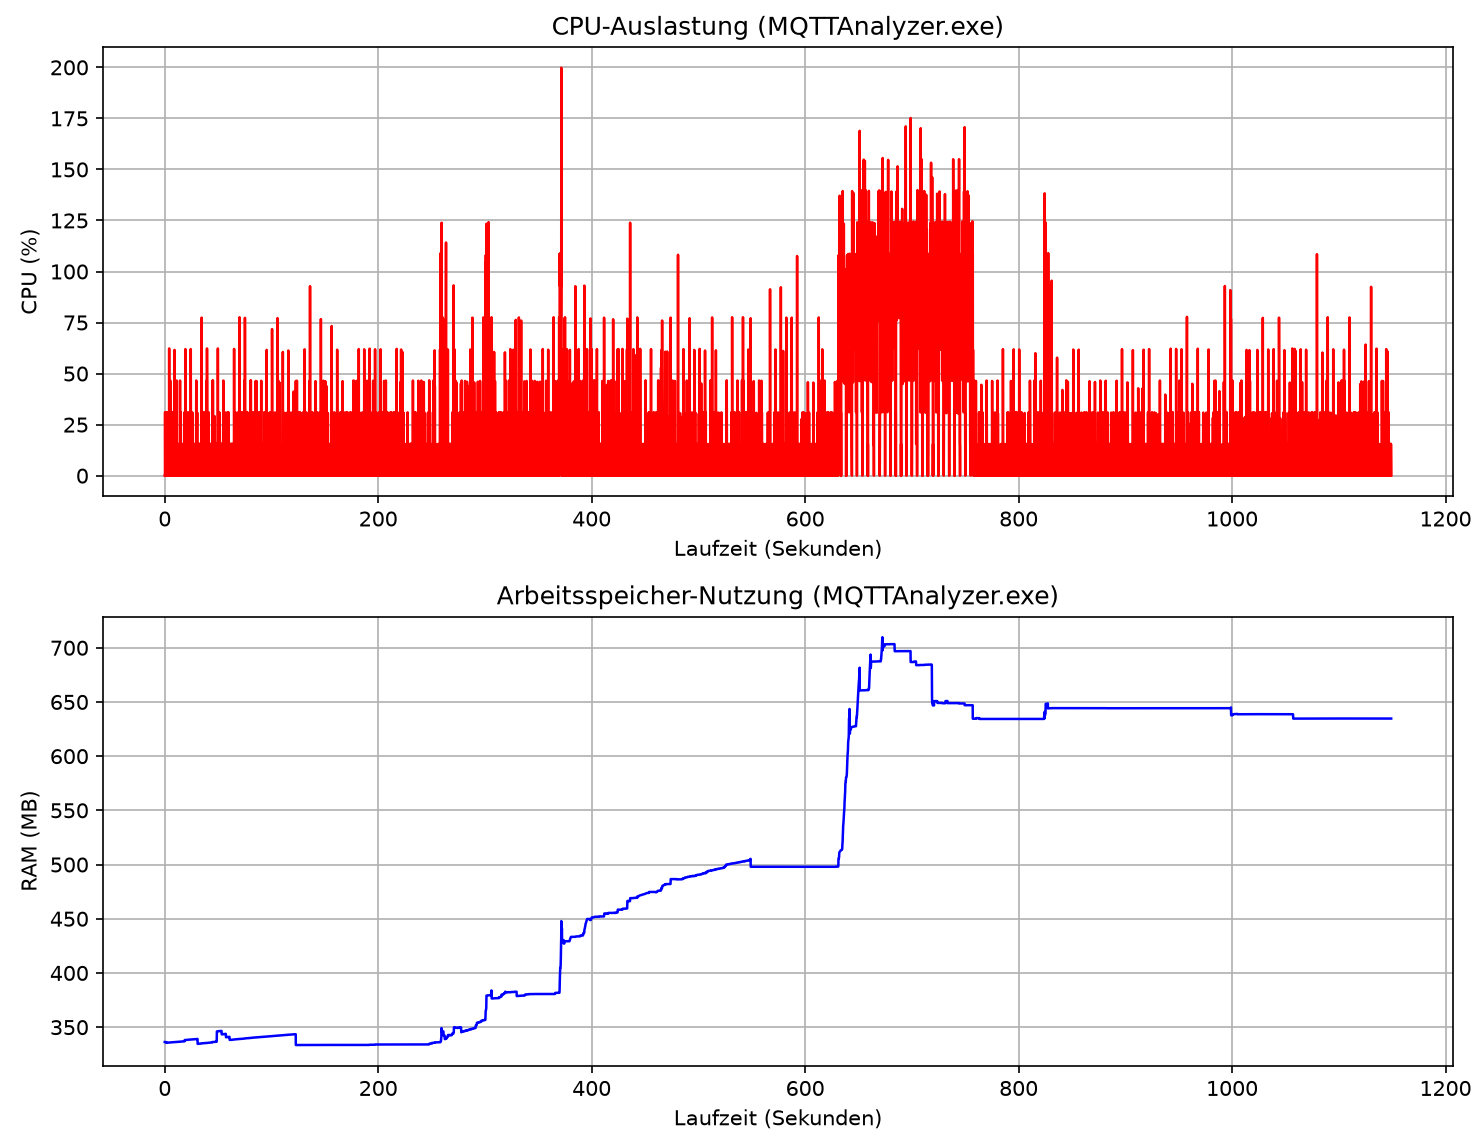
\includegraphics[width=0.8\textwidth]{images/Messwerte.png}
            \caption{Verlauf des Ram-Verbrauchs und der CPU-Auslastung in Abhängigkeit der Zeit}
            \label{fig:Messwerte}
        \end{figure}